\documentclass[main.tex]{subfiles}
\begin{document}
在物理学理论中,一切宏观物质体系都符合各个守恒律或基本物理定律,比如质量不灭(经典理论)、动量守恒、热力学定律等。但是我们仍然能够看到,不同的物质体系,在给予相同的外部刺激时,显示不同的响应。这说明守恒律并不足以确定物质体系的物理性质。本构方程(constitutive equation)或本构关系(constitutive relation)就是描述特定材料的两个物理量(尤其是运动学物理量和动力学物理量)之间的关系。本构关系必然不与守恒律相冲突,但要解决具体的物理问题,必须结合本构关系和守恒律来解决物理问题。仅靠守恒律就能解决的问题是很少见的,比如仅限于单个质点或理想刚体,且没有热传导的情况,因为在这种情况下体系的质量或质量分布是唯一决定动力学性质的特性。

\begin{figure}[ht]
    \centering
    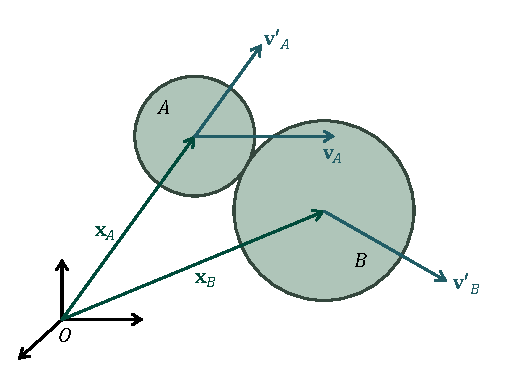
\includegraphics{images/I.1.1.pdf}
    \caption{刚性硬球碰撞问题。}
    \label{fig:I.1.1}
\end{figure}
\begin{example}
    完全弹性碰撞的运动规律是可通过守恒律直接得出的。考虑两个刚体圆球A与B质量分别为$m_\text{A}$、$m_\text{B}$,它们碰撞时位于$\mathbf{x}_\text{A}$、$\mathbf{x}_\text{B}$(如图\ref{fig:I.1.1}所示)。两球碰撞前、后的速度分别记为$\mathbf{v}_\text{A}$、$\mathbf{v}_\text{B}$、$\mathbf{v}_\text{A}^\prime$和$\mathbf{v}_\text{B}^\prime$。若它们之间发生的是完全弹性碰撞,能量不转化成热或内能,不考虑重力,则碰撞前后的能量守恒仅限于动能守恒,即有
    \[m_\text{A}\left\|\mathbf{v}_\text{A}\right\|^2+m_\text{B}\left\|\mathbf{v}_\text{B}\right\|^2=m_\text{A}\left\|\mathbf{v}_\text{A}^\prime\right\|^2+m_\text{B}\left\|\mathbf{v}_\text{B}^\prime\right\|^2\]
    若再与动量守恒式联立,
    \begin{align*}
        m_\text{A}\mathbf{v}_\text{A}+m_\text{B}\mathbf{v}_\text{B}                                                                             & =m_A\mathbf{v}_A^\prime+m_\text{B}\mathbf{v}_\text{B}^\prime                                                                                           \\
        m_\text{A}\left(\mathbf{x}_\text{A}\times\mathbf{v}_\text{A}\right)+m_\text{B}\left(\mathbf{x}_\text{B}\times\mathbf{v}_\text{B}\right) & =m_\text{A}\left(\mathbf{x}_\text{A}\times\mathbf{v}_\text{A}^\prime\right)+m_\text{B}\left(\mathbf{x}_\text{B}\times\mathbf{v}_\text{B}^\prime\right)
    \end{align*}
    则只要已知$\mathbf{v}_\text{A}$和$\mathbf{v}_\text{B}$就可以预测$\mathbf{v}_\text{A}^\prime$和$\mathbf{v}_\text{B}^\prime$。
    \begin{align*}
        \mathbf{V}_\text{A}^\prime & =\mathbf{v}_\text{A}-\frac{2m_\text{B}}{m_\text{A}+m_\text{B}}\frac{\left(\mathbf{v}_\text{A}-\mathbf{v}_\text{B}|\mathbf{x}_\text{A}-\mathbf{x}_\text{B}\right)}{\left\|\mathbf{x}_\text{A}-\mathbf{x}_\text{B}\right\|^2}\left(\mathbf{x}_\text{A}-\mathbf{x}_\text{B}\right) \\
        \mathbf{v}_\text{B}^\prime & =\mathbf{v}_\text{B}-\frac{2m_\text{A}}{m_\text{A}+m_\text{B}}\frac{\left(\mathbf{v}_\text{B}-\mathbf{v}_\text{A}|\mathbf{x}_\text{B}-\mathbf{x}_\text{A}\right)}{\left\|\mathbf{x}_\text{B}-\mathbf{x}_\text{A}\right\|^2}\left(\mathbf{x}_\text{B}-\mathbf{x}_\text{A}\right)
    \end{align*}

    但若两球发生非完全弹性碰撞,那么要从碰撞前的速度预测碰撞后的速度,需要再知道碰撞的恢复系数,它被表观地定义为
    \[e\equiv\frac{\left\|\mathbf{v}_\text{B}^\prime-\mathbf{v}_\text{A}^\prime\right\|}{\left\|\mathbf{v}_\text{B}-\mathbf{v}\text{A}\right\|}\]
    它是属于这于体系本身的特征。这一例子说明,只要稍微不那么理想的问题,都无法仅用守恒律,而不问体系具体特性,就实现这一问题的理论预测。
\end{example}

\begin{example}
    考虑一个封闭的气体体系的绝热压缩过程,我们希望求该过程中单位体积变化导致多大的温度变化。假设过程是可逆的,即$\updelta Q=T\mathrm{d}S=0$。其中$updelta Q$是可逆过程的热量变化,$T$是温度,$S$是熵。由于体系是气体,其状态可独立由$T$和体积$V$完整的确定。因此$S=S\left(T,B\right)$,对期进行全微分,并利用Maxwell关系,有
    \begin{align*}
        \mathrm{d}S                                           & =\left.\frac{\partial S}{\partial V}\right|_{T}\mathrm{d}V+\left.\frac{\partial S}{\partial T}\right|_{V}\mathrm{d}T \\
                                                              & =p\beta\mathrm{d}V+\frac{C_V}{T}\mathrm{d}T                                                                          \\
                                                              & =0                                                                                                                   \\
        \Leftrightarrow T^{-1}\frac{\mathrm{d}T}{\mathrm{d}V} & =-\frac{\tilde{\beta}\left(T,V\right)}{C_V\left(T,V\right)}
    \end{align*}
    其中$\beta\equiv p^{-1}\left.\frac{\partial p}{\partial V}\right|_{V}=\tilde{\beta}/p$是压力系数,$C_V\equiv\left.\frac{\updelta Q}{\mathrm{d}T}\right|_{V}$是等容热容。它们都是与气体本身性质有关的响应函数。上列结果说明,仅通过热力学基本定律和微积分关系,只能得到上式,它是一个关于函数$T\left(V\right)$的常微分方程。想要知道系体的(可逆)绝热压缩过程中,单位体积的变化导致多大的温度变化(即函数$T\left(V\right)$的形式),必须知道$C_V\left(T,V\right)$和$\tilde{\beta}\left(T,V\right)$的函数形式,而后者则要求已知体系的状态方程$p=p\left(T,V\right)$。

    比如,若该气体是理想气体,则有$p=nRT/V$,其中$n$是气体分子的物质的量,$R$是气体常数。由此可知$\tilde{\beta}=pT^{-1}$。此外,由理想气体的性质,$C_V$是常数,但仍需确定其数值(比如还需已知气体分子的结构等信息,或由实验确定)。这时,上列方程变成关于函数$T\left(V\right)$的可直接求解的常微分方程,结果是
    \[T=T_0\left(\frac{V}{V_0}\right)^{nR/C_V}\]

    类似地,若该气体是范德华气体,则有$p=\frac{nRT}{V-bn}-\frac{an^2}{V^2}$,其中$a$、$b$是范德华气体状态方程的参数。由Maxwell关系可得
    \[\left.\frac{\partial C_V}{\partial V}\right|_T=T\left.\frac{\partial^2p}{\partial T^2}\right|_V=0\]
    故范德华气体的等容热容是温度的函数,$C_V=C_V\left(T\right)$,其具体形式仍需确定。此外,由状态方程可知
    \[\tilde{\beta}=\left.\frac{\partial p}{\partial T}\right|_V=\frac{nR}{V-bn}\]
    故范德华气体的约化压力系数是形如上式的关于体积的函数,$\tilde{\beta}=\tilde{\beta}\left(V\right)$。上列方程仍是一个可解的常微分方程。
\end{example}
\end{document}
